\section{Design}
\label{sec:design}

In this section we describe the design of RCuckoo, a fully
disaggregated lock-based cuckoo hash table in which clients
communicate with passive memory servers over reliable RDMA connections
using exclusively 1-sided operations.  We first describe our table
design and protocol to read and modify the contents of the table.  In
the common case, reads complete in one or two round trips while update and
delete operations require two.  Then we introduce a locality-enhanced
hashing algorithm and show how it enables our protocol to perform
inserts in a small number of round trips.  Finally, we discuss
lock-table practicalities.  For simplicity, we describe our design in
the context of a single memory server, but it is straightforward to
shard a large hash table across multiple servers (with a minor tweak
to the hashing function, see Section~\ref{sec:dephash}).
%We close with a discussion of how RCuckoo detects and recovers
%from client failures.

\subsection{Datastructures}
\label{sec:table-design}

\begin{figure}[t]
    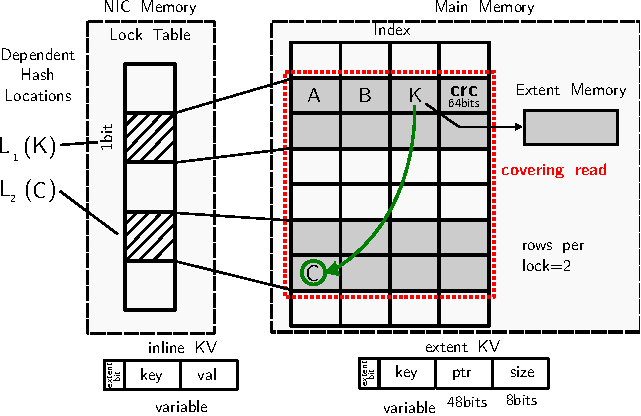
\includegraphics[width=0.99\linewidth]{fig/table-diagram.pdf}
\vskip -0.5em
    \caption{RCuckoo's datastructures showing an insert of the key $K$ as it displaces $C$.}
    \label{fig:table-diagram}
    \vskip -1.5em
\end{figure}

Figure~\ref{fig:table-diagram} shows RCuckoo's index and lock table
(both maintained at the remote memory server) during an insertion of
key $K$.  The index table (right) is a single region of
RDMA-registered main memory divided into rows of fixed-width entries.
Each row contains $n$ associative entries (3 in this figure, we use 8
in practice) and terminates with an 8-bit version number and 64-bit
CRC (that is computed over the entire row including version number).
Clients access the index table using 1-sided RDMA reads and writes;
CRCs facilitate lock-free reads as each row can be self-verified while
version numbers enable clients to detect if a row has been modified.
Locks (stored in a bit vector in NIC memory, shown on the left) each
protect a tunable number (here, two; 16 in our experiments) of index
rows.  Clients perform lock acquisition and release with RDMA
compare-and-swap (CAS) operations.  Specifically, RCuckoo leverages
masked CAS (MCAS) operations~\cite{rdma-masked-cas,sherman} to obtain
multiple locks simultaneously while avoiding false sharing.

%by polling CRCs which is used to detect if a client
%has failed while holding a lock (Section~\ref{sec:fault-tolerance}).

As shown at the bottom of the figure, Table entries contain
either inlined key/value pairs which are used by default
(and signified by a 0 MSB) or a key and 48-bit pointer to an
extent entry for larger values. We use 8-byte entries in our
experiments, with 4-byte keys and 4-byte values.
%\footnote{The performance of larger values is shows in Section~\ref{sec:entry_size}}.
%~\footnote{Inlined entries perform better on small key
%value pairs}.
Extents are located in preallocated, per-client regions of
server memory to avoid contention on inserts.


%%
%When an entry is modified its row's version number is
%incremented and its CRC is recalculated including the
%updated version number.

%%

% The lock table
% (Section~\ref{sec:locking}) is shown on the left~\todo{add
% virtual table}. 
% ~\todo{We leave resizing to future work.}. 
%%
% \textbf{Client Caching:}
%%
\todo{describe memory allocation}

\subsection{Operations}

We detail the operations supported by RCuckoo below;
Figure~\ref{fig:message_diagram} visualizes the corresponding message
exchanges. 

\subsubsection{Reads} 
\label{sec:reading}


RCuckoo is designed to facilitate lock-free, single round-trip reads
for small values as they are the dominant operation for key/value
stores in many data centers~\cite{rocks-db-workload,facebook-memcached}. To
read the value associated with a given key clients calculate the
potential table locations for the key's entry (using the hash
functions described in the next subsection) and issue RDMA reads for
both rows simultaneously.  Because all operations between a client and
a given server travel over a reliable connection, they are
intrinsically ordered, but in our description we will only call out
when a particular ordering among a batch of messages is required.


Moreover, as we discuss below, if the rows are
located sufficiently close together, it can be beneficial for the
client to issue a single \emph{covering read} that returns the
contents of both rows---as well as intervening and potentially
surrounding ones---in a single request.
In our experiments RCuckoo clients issue a single, large read rather than two small reads if the locations are within 148 bytes of each other (i.e., adjacent rows)
%within
%close to one another in the table to
%reduce tail latency. We use
%128 bytes of each other
as our parameter sweeps show it has a negligible
increase in latency over smaller RDMA requests
(Figure~\ref{fig:rdma-benchmarks}(b)) and provides substantial
improvement for insert operations.  (If bandwidth is not a concern, we
find that a 2-KB threshold can deliver a further 3\% boost to insert
performance, but the resulting read amplification is significant.)


\begin{figure}[t]
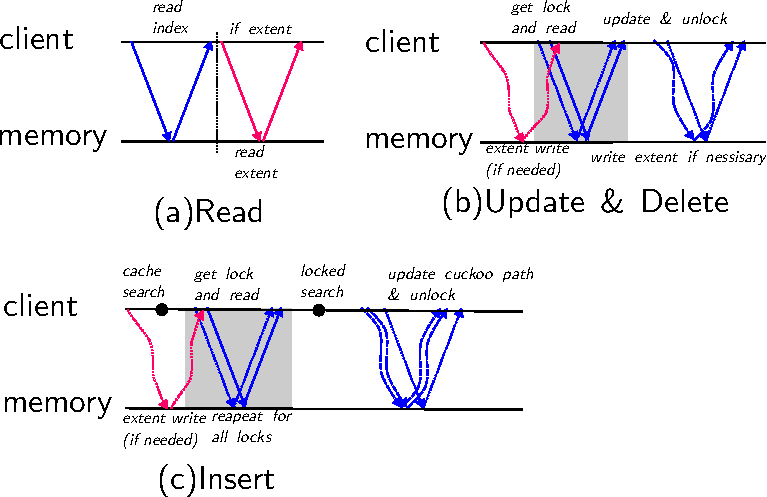
\includegraphics[width=0.99\linewidth]{fig/message_diagram.pdf}
%%
\caption{RCuckoo's protocol for reads, inserts, deletes and
updates. Blue lines are index accesses, and red lines are
extent accesses. Solid lines are reads, dotted lines are
CAS, and curved dashed lines are writes.}
%%
\label{fig:message_diagram}
\vskip -1em
\end{figure}


A read is successful if either row contains an entry with the desired
key and the row's CRC is valid. An invalid CRC indicates a torn write
or rare failure case, in which case the operation is retried
(see Section~\ref{ss:fd}).  As shown in
Figure~\ref{fig:message_diagram}(a) inlined reads are complete after
one round trip, while reads for large values require a second round
trip to retrieve the extent.


\subsubsection{Updates and deletes}

Updates and deletes, like reads, access only two locations in the
index table, but require a client to acquire the associated locks.
Due to RCuckoo's locality enhancement, it is usually possible to
attempt to acquire both locks in a single MCAS operation
(Section~\ref{sec:locking}).  If so, the client issues read(s) for the
corresponding rows of the index table immediately afterwards but in
the same batch of operations.\footnote{Because the lock table is
located in NIC memory, RCuckoo clients can employ \texttt{SEND\_FENCE}
on reads batched with lock acquisitions to ensure consistency without
incurring a performance penalty.}  In the rare case that the locks
must be acquired independently---necessitating an additional round
trip---the reads are batched with the second lock request.

Assuming
successful lock acquisition and valid reads, the operation can proceed
if the key is present in either location.  In a single (ordered) batch
of operations, the client first writes the updated/freed entry and
recomputed row version and CRC before releasing the locks. When
updating values stored in extents, clients store the value to a new
extent in an RDMA write that is batched with the lock acquisition
requests to avoid additional round trips.  Deletes of extent-based
values simply mark the entry for later garbage collection.
Figure~\ref{fig:message_diagram}(b) shows that most uncontested operations
complete in two round trips; clients retry acquisitions until they succeed or detect a failed client.
%(see Section~\ref{ss:fd}).

\todo{How does extent garbage collection work?}

% If reading both
% locations as a single read is greater than 128 bytes, the
% read is issued as two parallel reads to individual rows
% similar to prior work without locality
% optimizations~\cite{pilaf, race}. Inlined entries are read
% in a single round trip, while extent entries require two
% (Figure~\ref{fig:message_diagram}).

% Reads are performed locklessly. Readers recalculate and
% check the rows CRC to validate the read. Clients reissue the
% read if the CRC is invalid as it is likely due to the read
% encountering a torn write. Continuously invalid CRC's can be
% the result of a client failure mid write. Our algorithm for
% detecting and repairing the table from partially completed
% writes is described in Section~\ref{sec:table-repair}.

\subsubsection{Insert}
\label{sec:insert}

Inserts are challenging because concurrent operations might result in
cuckoo paths that collide.  Rather than face the prospect of having to
unravel a partially completed insert upon collision, RCuckoo clients
compute a complete cuckoo path ahead of time and then acquire locks on
all the relevant rows to ensure its success.  Moreover, to facilitate
recovery from client failures, an insert is performed by cuckooing
elements one at a time, starting by moving the last entry in the path
to the empty location, and then replacing it with the previous
entry in the path, and so on until the new entry is inserted in its primary location.


To speed up cuckoo-path searches, RCuckoo clients keep a local,
RDMA-registered cache of (relevant portions of) the index table.
Clients validate---and, if necessary, update---their cache at each
step of the insert operation as explained below, so stale cache
entries do not impact correctness, only performance.



%% Insertions are the highest complexity operation because
%% client caches are not synced with remote memory. Without
%% knowing the state of remote memory clients can neither
%% calculate valid cuckoo paths locally and nor determine which
%% locks they will require to perform an insertion.



% \textbf{Memory Allocation:}
% %%
% \sg{Help alex, I need to remove this section but I don't
% quite know how to talk about memory allocation or extent
% memory}
% %%
% Prior work has focused on different memory allocation and
% hash table resizing schemes. Sherman~\cite{sherman} uses an
% allocated thread located on the memory node,
% Fusee~\cite{fusee} uses a two tired memory allocation in
% which large blocks of memory are allocated on the memory
% nodes and fine grained allocation is performed on the
% clients. Clover~\cite{clover} statically partitions memory
% into large client regions prior to execution and hash
% clients entirely manage the space themselves. Network based
% allocators such as MIND and Clio~\cite{mind,clio} have
% demonstrated the feasibility of high performance
% disaggregated allocators, while some have called for
% allocators to be built into RDMA~\cite{prism}. We allocate
% memory using the same scheme as Clover, as it is simple to
% implement and adds no additional overhead. We view memory
% allocation as a hard orthogonal problem to the design of
% disaggregated indexes and have designed our system
% acrostically to the allocator.

At a high level an insert operation proceeds in three phases.  RCuckoo
clients start by identifying a potential cuckoo path using only the
contents of their local table cache.  Clients then simultaneously
attempt to acquire the locks for and update their cache of the rows
that comprise the candidate path.  Using only the contents of their
newly updated local cache, clients conduct a second search to confirm
that a candidate path---either the initial guess or an alternative
that similarly consists only of currently locked rows---exists.  If
so, the insert is performed; if not, the client releases its locks and
retries the operation.

\textbf{Speculative local search:} As noted in
Section~\ref{sec:cuckoo-back} identifying a viable cuckoo path for
insertions requires multiple dependent reads.  RCuckoo attempts to
limit the number of remote operations by first conducting a
speculative local search. Prior to contacting the server, RCuckoo
clients search the contents of their local table cache to build a
speculative cuckoo path.  As with prior work, we use breadth-first
search (BFS) to identify short paths in an attempt to minimize
bandwidth and locking overhead~\cite{cuckoo-improvements}.  If the
client cache is empty the degenerate path is presumed, i.e., that the
key will be inserted into either its primary location
without the need for any cuckooing.  Obviously, speculative cuckoo
paths are most useful when client caches are fresh---often due to a
failed prior attempt to insert the same key.

% Because of
% locality hashing there is a high probability that a valid
% insertion path can be found in buckets near a speculative
% path, even if the clients cache is stale.

\textbf{Cache synchronization:} Armed with a potential
cuckoo path, clients identify the set of locks necessary to
protect the relevant rows.  
%%
Approximately 99\% of paths can be locked with a single MCAS
operation (Figure~\ref{fig:locality-hashing}(c)); longer
paths acquire locks in groups (Section~\ref{sec:locking}).
%%
Immediately after, but in the same batch of RDMA operations
as each attempt to acquire (a subset of) the locks, clients
synchronize their local cache by issuing reads for (at
least) all of the rows covered by that set of locks.  In
general, locks cover multiple rows, so this will be a
superset of the rows necessary for the identified path.
Note that if lock acquisition is successful, the values
returned by the read of the corresponding rows---and, thus,
the client's local cache of those rows---will remain
synchronized until the lock is released.

Figure~\ref{fig:table-diagram} shows an example insert
operation where the client updated its cache of the section
of the index table outlined by the dashed red line using a
single covering read.  Here, the primary row for $K$ is full
and the entry for key $C$ is being evicted its secondary
location.  Hence, the client has acquired locks
corresponding to the row where it hopes to insert the entry
for key $K$ as well as the row into which it plans to cuckoo
the existing entry for key $C$.  The rows shaded in gray are
synchronized because they are covered by the acquired locks,
while the intervening two (unshaded) rows are updated in the
client's cache, but their contents cannot be depended upon
without additional validation.  Rather, they may increase
the likelihood that a subsequent speculative search yields a
valid result.
% In this section we describe our protocol for reading,
% inserting, and performing updates and deletes to an
% RCuckoo hash table.  In principle, the cache can be
% maintained not just across retries but also across insert
% operations for different keys, but %Caches can be purged
% or persisted between requests %depending on a clients
% available memory.  %While theoretically %these caches
% could be persisted to improve performance our
% experimentation shows that performance gains are minimal %
% due to high churn in the cuckoo index lock granularity
% paired with %read strategy (Section~\ref{sec:insert}) has
% a far higher impact on %search success over caching
% (Section~\ref{sec:search_success}).

\begin{figure*}[t]
    \centering
%    \begin{subfigure}{0.3\linewidth}
%        \begin{align*}
%            L_1 &= h_1(k) \\
%            L_2 &= L_1 + (h_2(k)\mod f^{f + log_2(h_3(k))})
%        \end{align*}
%        % \caption{}
%        % \label{fig:hash_factor}
%    \end{subfigure}
    \begin{subfigure}{0.3\linewidth}
        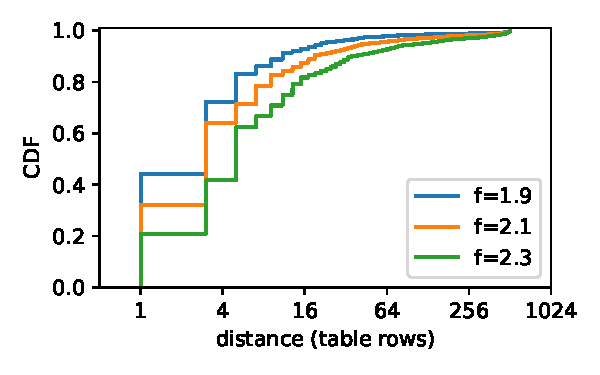
\includegraphics[width=0.99\linewidth]{fig/hash_factor.pdf}
        % \label{fig:hash_factor}
        % \caption{}
    \end{subfigure}
    \begin{subfigure}{0.3\linewidth}
        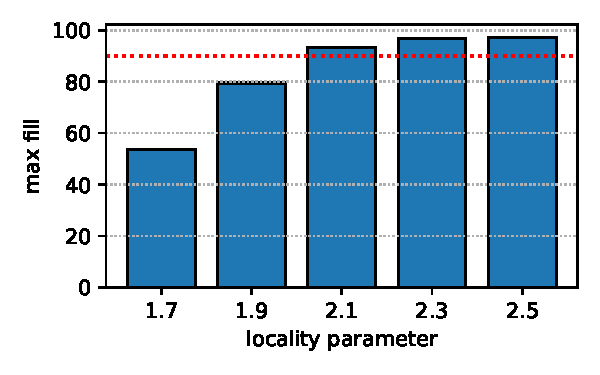
\includegraphics[width=0.99\linewidth]{fig/hash_fill.pdf}
        % \label{fig:hash_fill}
        % \caption{}
    \end{subfigure}
        \begin{subfigure}{0.3\linewidth}
        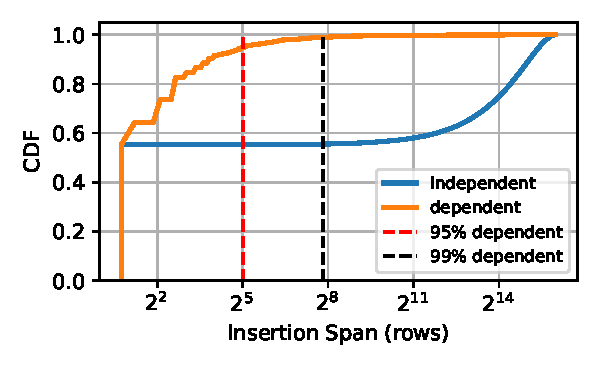
\includegraphics[width=0.99\linewidth]{fig/insertion_span.pdf}
        % \label{fig:insertion_span}
        % \caption{}
    \end{subfigure}
    \vspace{-1em}
    \caption{
 %   \textbf{(a)} Dependent hashing for factor $f$.
    \textbf{(a)} CDF of distances between cuckoo locations for different locality settings using RCuckoo's dependent hashing.
    \textbf{(b)} Achieved maximum fill percentage for different locality settings. 90\% fill indicated by dashed red line.
    \textbf{(c)} CDF of cuckoo spans for dependent and independent hashing. A cuckoo span is the distance between the smallest and largest index in a cuckoo path.
    }
    \label{fig:locality-hashing}
\vskip -1em
\end{figure*}


\textbf{Second search:} If all the lock acquisitions are successful,
the client validates that the initial path remains valid.  Under an
insert-heavy workload, however, speculative cuckoo paths are
frequently stale.  Yet, a valid cuckoo path may still exist within the
locked rows.  Hence, if the initial path is no longer viable, clients
perform a second search restricted to only the synchronized part of
its cache, i.e., rows for which they currently hold the lock.  In
either case, if a valid path is found the series of swaps and
version/CRC updates are calculated and issued as a batch of RDMA
writes, one row at a time, followed by (an ordered set of) lock
releases. If no valid path exists the client releases its locks and
tries again, conducting another speculative search on the updated
cache contents.

\todo{Lightly filled table optimization}

This entire process repeats until success, a client determines there
is no viable cuckoo path (at which point the insert operation returns
an error indicating the table is full), or a failed client is detected.  Given the fully-disaggregated
context we assume the index table will be initially provisioned at its
maximum size; we defer resizing to future work.
%\todo{describe resizing}
% During development we
% experimented heavily with guided A* search but found that it
% only offered improvements over BFS when the table was over
% 95\% full due to the setup overhead of A* and the fact that
% most paths are short.
If cuckoo paths were to randomly span the table it is unlikely that an
alternate valid path would exist within the locked rows when
speculation fails.  In the next subsection, however, we describe how
RCuckoo uses dependent hashing to dramatically increase the likelihood
that an alternate path exists using rows surrounding those identified
by the speculative search.
%Our evaluation measures the success
%rate of insertions as a function of lock granularity
%(Section~\ref{sec:search_success}).


% However, as noted
% there is high probability that a valid path can be found
% within the locked rows due to hash locality. 
%  during second search each update and CRC along the
% path along with unlock messages are batched together. 




\subsection{Locality}


%% Randomly spread cuckoo paths take many round trips to find and lock.
%% Similarly, reads require reads of both the potential locations for a
%% given key.  

In a traditional cuckoo hash, the two locations for a given key are
deliberately independent which allows the table to be filled quite
full before inserts begin to fail. 
%
In RCuckoo the distance between keys' two cuckoo hash locations is a
tunable parameter.
We show experimentally that an optimal locality
setting can dramatically decrease the number of round trips required
to perform inserts in RCuckoo while maintaining high (90\%+) fill
maximum factors.

Increased locality has two direct benefits: it
increases the probability that both of a keys' locations can be read
with a single covering read---which updates more of a client's local
cache, improving the likelihood that failed insert operations will
succeed upon retry---and decreases the number of MCAS operations
necessary to acquire the relevant locks.  It also reduces the region
of the index table likely to be spanned by cuckoo paths, which speeds
up inserts, but leads to hot spots that limit the table's expected
maximum fill factor.  


%\subsubsection{Dependent hashing}
\label{sec:dephash}


%% \begin{figure*}[t]
%%     \centering
%%     \begin{subfigure}{0.3\linewidth}
%%         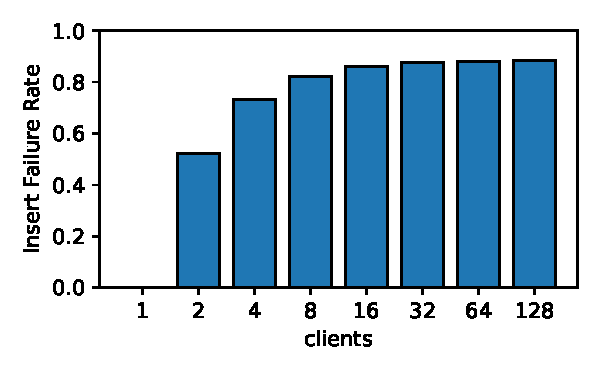
\includegraphics[width=0.99\linewidth]{fig/optimistic_failures.pdf}
%%         % \label{fig:optimistic_failures}
%%         % \caption{}
%%     \end{subfigure}
%%     \begin{subfigure}{0.3\linewidth}
%%         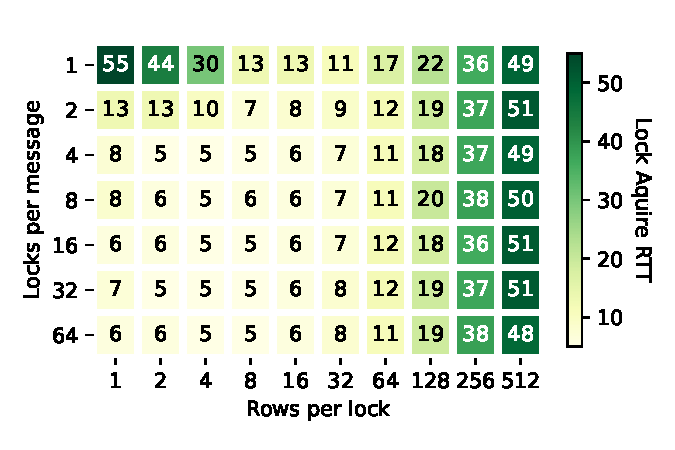
\includegraphics[width=0.99\linewidth]{fig/buckets_per_lock_vs_locks_per_message.pdf}
%%         % \label{fig:tbd}
%%         % \caption{}
%%     \end{subfigure}
%%     \vspace{-1em}
%%     \caption{
%%     \textbf{(a)} Failure rate of optimistic cuckoo insertions.
%%     \textbf{(c)} Round trips (99th percentile) on a table
%%     with 512 rows required per insert while filling a table
%%     to 95\%. 512 buckets per lock is a single global lock.}

%%     \label{fig:cuckoo-problems}

%% \end{figure*}

%Our hashing algorithm borrows from both cuckoo and hopscotch hashing
%to achieve tunable locality.


In RCuckoo, the primary location for a key is chosen uniformly at random,
while the second is offset from the first by 
uniformly random value drawn from a probabilistically bounded range, where the
range is likely to be relatively small.  We start with a base
hash\footnote{We use xxHash~\cite{xxhash} in our implementation.},
$h()$, and use it to implement three independent hash functions
$h_1()$, $h_2()$, and $h_3()$.  (In our implementation we use a
different salt for each of the three functions.)  We compute the two
locations $L_1$ and $L_2$ for a key $K$ as
\[ L_1(K) = h_1(K)\mod T, \]
\[ L_2(K) = L_1 + (h_2(K)\mod f^{f+\mathcal{Z}(h_3(K))})\mod T, \]
\noindent where $T$ is the size of the index table in rows,
$\mathcal{Z}(x)$ is the number of trailing zeros in $x$, and $f$ is a
parameter that controls the expected distance between the two hash
locations.  (In a sharded deployment, the second location is
restricted to the same shard by ``wrapping around'' the offset
accordingly.) The particular formulation is not important, but the
upshot is exponentially fewer keys have secondary locations at
increasing distances from their primary.  The latter aspect is crucial, as any
fixed bound on the distance between hash locations leads to low
maximum fill factors (on the order of 10--15\% in our experiments).

Figure~\ref{fig:locality-hashing}(a) shows the distance between hash
locations as a CDF for different values of $f$,
%% Setting .  using a third hash function $h_3(x)$
%% which generates a higher exponent at a logarithmic rate to determine
%% which locations will have large distances between them
%% %\footnote{The
%% %value of $h_3(x)$ is the sum of trailing zeros after calculating a
%% %keys 64bit hash value}
%% These few, but far apart hash locations
%% increase the max fill by alleviating hotspots in the table. While
%% searching for cuckoo paths with BFS these entries act as gateways for
%% paths to access less filled portions of the table.
while Figure~\ref{fig:locality-hashing}(b) shows that larger values of
$f$ enable practical fill factors for tables with 100~M entries. In
our evaluation we set $f=2.3$.  As shown in the figures, for index
tables with eight entries per row, RCuckoo delivers an expected max fill of
greater than 95\% with a 68\% probability that a key's locations are
located five or fewer rows apart.


Decreased distances between hash locations naturally lead to shorter
cuckoo paths when combined with our breadth-first search approach.
Using $f=2.3$ and a table size of 100-K rows,
Figure~\ref{fig:locality-hashing}(c) shows that when filling the table
to 95\% full, slightly more than half of insertions do not require any
cuckooing, and 95\% of insertions require cuckoo paths that span 32 or
fewer rows while nearly 99\% span 256 or fewer.  Conversely, with
independent hashing, insertions that require any cukooing at all
almost always result in spans of 2~K rows or more.
%This setting
%yields paths that will frequently fit within the rows returned by a
%covering read.
%
%\todo{I don't understand the independent lien---50\% have a span of 1?  Maybe remove for now?}

%% Locality provides an additional opportunity to reduce round
%% trips by reading additional buckets. If locks are close
%% together but not contiguous clients issue a \textit{covering
%% read} spanning all rows between each bucket. We use 512
%% bytes as a max threshold. Covering reads synchronize a
%% clients cache for non-locked rows. If the second search
%% fails to find a valid cuckoo path the next iterations
%% speculative search will benefit from the fresh read.
%% Figure~\ref{fig:table-diagram} illustrates a covering read
%% between keys $K$ and $C$.

% Speculative locks may not be sufficient to complete an
% insertion.  However, due to locality hashing there is a high
% probability that a valid path does exist in the neighborhood
% of the speculative locks. 
% If two speculatively locked rows
% are close enough together clients issues a single
% \textit{covering read} spanning both rows. Covering reads
% populate a clients cache and dramatically increase the
% probability that if the first speculative search fails, a
% subsequent search will succeed.  We set the max threshold
% for covering reads to 512 bytes in all our experiments.
% Figure~\ref{fig:table-diagram} illustrates an insertion of
% key $K$ displacing key $C$. Here the speculative search
% marked the rows for $C$ and $K$ to be locked. A covering
% read (red) spans the rows between both entries.

\subsection{Locking}

While RCuckoo reads are lock free, updates and especially inserts
depend critically on locking performance.

\subsubsection{Lock granularity}
\label{sec:locking}

\begin{figure}[t]
  \vskip -1em
    \centering
        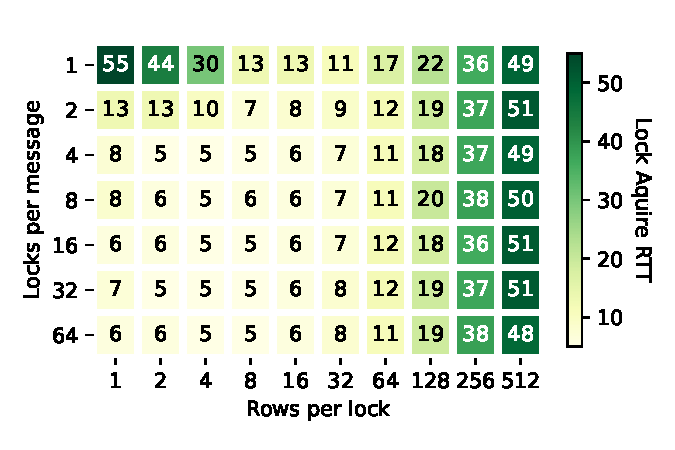
\includegraphics[width=0.99\linewidth]{fig/buckets_per_lock_vs_locks_per_message.pdf}
    \vspace{-1em}
    \caption{99th-percentile round trips required per insert in a 512-row table
    when filling to 95\%. 512 buckets per lock corresponds to a single global lock.}
    \label{fig:cuckoo-problems}

\end{figure}

Increased locality decreases the number of round trips required
for lock acquisition.
%Moreover, the required locks are also close to each other in the lock
%bit array.
Recall the lock table is a linear array of lock bits and each bit
locks one or more table rows.  As mentioned previously, RCuckoo
implements lock acquire and release using RDMA masked compare-and-swap
(MCAS) operations that can update 64 bits at a time.  To avoid
deadlock RCuckoo acquires locks in increasing order.  For any given
operation, clients group the necessary locks into the smallest number
of sets as possible (where each set is an attempt to acquire one or
more locks within a single 64-bit span) and issue MCAS operations one
at a time in order of their target address.  Clients continuously spin
on lock acquisitions and only move to the next MCAS operation after
the current one succeeds.  Due to this one-MCAS-per-round-trip
acquisition procedure, lock granularity is critical to performance.

If, as in Figure~\ref{fig:locality-hashing}(c), almost 99\% of cuckoo
spans are 256 rows or less, and each lock protects four rows, nearly
99\% of insertions can have their locks acquired with a single MCAS.
Of course, increasing the number of rows covered by a single lock can
lead to false sharing, forcing additional retries to acquire the
necessary locks.
%(In the extreme, there would just be one, global
%lock for the entire table.)  We conduct a parameter sweep to determine
%the best choice of lock granularity for our setting.
%
Figure~\ref{fig:cuckoo-problems} shows the results of a
representative experiment where 8 clients are concurrently
filling a 512-row table to 95\% full.  We report the
99th-percentile (i.e., the most expensive inserts when the
table is nearly full) number of round trips required to
acquire the locks necessary to perform an insertion as a
function of both lock granularity (i.e., number of rows per
lock, on the $x$-axis) and lock size (i.e., the number of
locks that can be accessed with a single MCAS operation, on
the $y$-axis---RCuckoo's single-bit locks correspond to 64
locks per message).

While there is some noise due to experimental variance, the far-right
column shows that a single global lock results in high contention (as
there is only one lock in the system, it does not matter how many
locks can be acquired per message).  Conversely, the top left corner shows
that, despite the lack of false sharing when a lock corresponds to
exactly one row, the inability to acquire more than one lock at a time
leads to a large number of round trips.  Under these conditions, the
sweet spot falls in the range of 2--16 rows per lock.  In our
experiments we use 16 rows per lock as, when combined with our choice of
$f$, only a single lock is required for the vast majority of insertions.

%
Clients may fail while holding locks, preventing other clients from
making progress.  As described in the next section, clients
independently detect such failures by setting a time out for lock
acquisition. To avoid false alarms, i.e., clients timing out due to a
slow-moving client (who might, for example need to acquire a long list
of contended locks), RCuckoo clients are given a bounded time to
acquire all their locks. If a client takes longer than this time to
acquire all of its locks it releases all held locks and restarts the
(timer and) acquisition process, hopefully allowing other clients to
complete their own acquisitions.


\subsubsection{Virtual locks}

While Figure~\ref{fig:cuckoo-problems} suggests that RCuckoo could
employ larger locks (e.g., 8--16-bits per) without increasing the
number of round trip times required to acquire them, there is an
additional design constraint that drives our choice of single-bit
locks.  Specifically, to improve locking performance, RCuckoo locates
the lock table in NIC device memory which delivers $3\times$ higher
throughout on contented addresses than host memory (see
Figure~\ref{fig:rdma-benchmarks}). It is also lower latency as
operations to device memory avoid a PCIe round trip.  Unfortunately, NIC memory is limited (to
256~KB on our ConnectX-5s), so this choice bounds the size of the lock
table and drives our single-bit design.

Moreover, to allow RCuckoo to support tables with more than 64~M rows,
we implement a \textit{virtual} lock table where multiple logical
locks map to a single physical lock.  Concretely, we map a logical
lock $l$ drawn from a table of size $L$ to a physical location $p$ in
a bit-array of size $P$ by computing $p = l \mod P$.  Mapping multiple
virtual locks to a single physical lock introduces yet another source
of false sharing, but allows us to support arbitrarily large tables.
When employing virtual locking, clients performing an insert first map
rows to virtual locks, then to physical locks, then sort them into
groups.

% Using locks rather than opportunistic concurrency halves the
% latency of reads from two to one round trip. Opportunistic
% updates commit changes by atomically updating a pointer
% (with CAS) in the hash index to point to a new value. Both
% the index, then the value must be read for each operation.
% Values can not be inlined in the index as they are limited
% to the 64bit width of CAS. RCuckoo uses locks to enable
% inlined entries which can be read in a single round trip.
% Locks introduce multiple challenges such as scalability,
% deadlocks and fault tolerance each of which is discussed
% below.


%%




\section{Fault tolerance}
\label{sec:fault-tolerance}

In keeping with the rest of its design, RCuckoo handles failures in a
fully disaggregated manner as well.  We depend upon the RDMA hardware
to handle network failures and focus exclusively on fail-stop client
behavior.  Server failure can be addressed by employing client-driven
replication on top of RCuckoo.  While there may be opportunities to
integrate replication into RCuckoo itself, we defer such an
exploration to future work.  In RCuckoo, client failure is only of
concern if the failure occurs in the middle of a mutating operation
(i.e., update, delete, or insert); hence, RCuckoo detects client
failures by noticing that a pending mutation does not complete in a
timely fashion.  Any client that encounters such a situation endeavors
to recover the stranded lock and repair the impacted portion of the
index table.
%
%to prevent false failure detection. Our complete
%fault detection and recovery mechanism is described in
%Section~\ref{sec:fault-tolerance}.
%
%Specifically, clients acquire repair leases to reclaim the locks of
%failed clients and then perform the operations required to return the
%table to a valid state. In this section we
The remainder of this section describes how RCuckoo clients detect
faults, reclaim stranded locks, and, if necessary, repair the index
table.  Finally, we discuss additional measures that can
be employed to prevent stale writes if desired.

%, and prevent delayed
%RDMA writes issued by (assumed-to-be) failed clients from corrupting the table.

\subsection{Failure detection}
\label{ss:fd}
%\todo{note that we don't know who has the lock or when they got it}

Clients detect failures by setting a timeout when attempting repeated
lock acquisition or read requests.  Because RCuckoo operations are
designed to require only a few round trip times, a client performing a
successful mutating operation will complete and release its locks
extremely rapidly.  Conversely, a client that is unable to acquire all
the locks required for an insert operation releases those they do hold
before trying again.  Hence, it is extremely unlikely that repeated
attempts to acquire a lock or perform an untorn read will fail
continuously.

Of course, there is a possibility that a given row is highly popular,
leading to high lock contention and/or repeatedly torn reads.
Clients distinguish this case by consulting the CRC for the row they
are unable to successfully read or lock.  Because each mutation
increases the version number, even updates that replace an entry with
the same value will result in a different CRC.  Clients declare a
false positive and restart their failure timer if a CRC changes
between attempts.

We expect client failures to be relatively rare, so set
%\todo{talk about the actual timeout value} We view failures
%as a rare but essential component of our protocol. As such
our fault timeout conservatively. Failure timers must allow for
worst-case locking time, second-search time, and RDMA message
transmission time. We bound locking time;
%(Section~\ref{sec:locking});
search and message propagation are both measured in single-digit
microseconds on our testbed.  To guard against the possibility that
network conditions lead to high rates of RDMA retries we set
the maximum RDMA operation retry number to three.  In
this context, we set the failure timeout to 100~ms in our experiments,
orders of magnitude above the 99th-percentile insert time
of 50$~\mu$s.


\subsection{Repair leases}
%\todo{mention repair lease table}

RCuckoo recovers stranded locks one lock at a time; if a client fails
holding multiple locks recovery may be conducted by multiple clients
at different times depending on their access patterns.  RCuckoo's lock
table does not maintain records of ownership, so there is no way to
``transfer'' lock ownership from the failed node to a recovery node in
the table itself.  Instead, clients acquire a \emph{repair lease} that
grants exclusive permission to reclaim locks on a region of the index
table. The index table is broken into $n$ regions so repairs can be
executed in parallel.

\begin{figure}[t]
%  \vskip -1em
    \centering
        
\includegraphics[width=0.99\linewidth]{fig/lease.pdf}
 %   \vspace{-1em}
    \caption{Format of a repair lease table entry}
    \label{fig:lease}
   \vspace{-1em}
\end{figure}

Figure~\ref{fig:lease} shows the format for entries in
RCuckoo's lease table, maintained in RDMA-registered main memory on
the server.  Lease entries contain the lease holder's queue pair ID
(which RDMA ensures is unique for a given server), a set bit, and a
counter (incremented on each acquisition).  A lease is considered free
if the set bit of the current entry in the lease table is zero.
Clients attempt to acquire the lease using RDMA CAS operations to
ensure mutual exclusion.
%Failures
%while holding a lease are easier to detect than normal locks as a
%lease's owner and liveness are tracked within it.
Upon successful acquisition, a client completes the repair (described
below) and then relinquishes the lease by clearing the set bit.
Leases are revoked (to handle the case of a failed recovery node)
using a timeout mechanism similar to normal locks.  If a client times
out while attempting lease acquisition it claims it for itself (again,
using CAS to resolve any races) and marks the lease holder as failed
(see Section~\ref{sec:stale-writes}).
%A lock is reclaimed once a client
%both times out on a lock and acquires the locks repair lease.


\subsection{Table repair} 
\label{sec:table-repair}

%Our table design ensures that clients can perform repairs
%and recover from all states a failed client may have
%created.

All modification operations write new entries as a cuckoo path;
updates and deletes have a path of length one.  As described in
Section~\ref{sec:cuckoo-back} cuckoo paths are executed by first
claiming an open entry at the end of the path and proceeding backward
along the path, cuckooing entries forward one-by-one until the new
entry is written at the beginning of the path.  Client failures can
occur at any point along an insertion path; a failed client can leave
the table in one of four distinct states based on how far along it was:
\begin{enumerate}[itemsep=1pt]
\item{A duplicate entry exists and one has a bad CRC,}
    \item{A duplicate entry exists and both have correct CRCs,} 
    \item{No duplicate exists but one row has a bad CRC, or}
      \item{No duplicate exists and no rows have a bad CRC.}
\end{enumerate}
\noindent The last case can occur if a client fails prior to issuing
any updates to the table or if it fails after updating all the rows
but before releasing the locks.  In either case recovery is trivial: a
client with the repair lease can simply unlock the stranded lock.
Recovery from the other three cases requires modification to the index
table.

To repair the table a client first detects in which state the table is
and then transitions the table forward through the states with a
deterministic sequence of operations so that failures during recovery
can be repaired by a subsequent client. A client determines the state
by issuing reads to all rows protected by the stranded lock.  It then
proceeds one-by-one through each entry within the rows, checking both
hash locations for the corresponding key (one of which may not be in
the locked rows) for duplicates or a bad CRC.  Because RCuckoo updates
one row per RDMA write, there can be at most one duplicate or bad CRC.

Clients repair the table by moving though the states one step at a time.
%Corrections are issued as a batched sequence of three or fewer writes
%as follows:
To move from state 1 to 2, the client writes a new CRC for
the bad duplicate.  The table can be transitioned from state 2 to 4 by
clearing the duplicate entry in the second (i.e., pointed to by
$L_2(K)$) location. Finally, the table can be transitioned from state
3 to 4 by recalculating and writing a new CRC to the impacted
row. After a client has issued its repair sequence it unlocks the
reclaimed lock and returns its lease.

From a correctness perspective, once all rows have a valid CRC and
there are no duplicates, the table is usable again.  Clearly the new
value being inserted into the table by the failed client is lost, but
this is indistinguishable from the case that the client failed before
attempting the insert.  If the client was in the middle of cuckooing
values up the path, a subset of the values were moved from their
primary cuckoo location to their secondary location, but reads check
both locations in any case, so the entry will still be located.
Finally, because duplicate entries are freed, no space in the table is
lost.

\subsection{Preventing stale writes}
%%
\label{sec:stale-writes}
%%

The one remaining concern is that a supposed-failed client could
just be slow, and may yet attempt to complete its cuckoo path despite
the fact that its locks were reclaimed.
%(While
%RCuckoo clients abort insert operations if they take too long to
%acquire the required locks, they proceed to completion regardless of
%long it takes to issue the updates.)
Our failure timeout is
deliberately set many orders of magnitude larger than the expected
operation completion time, but we cannot completely rule out the
possibility.  Ideally, RCuckoo could ensure that clients deemed to have
failed by the failure detector are prevented from issuing further
operations to the table without manual intervention (e.g. a reboot).

%% An RDMA connection must be closed, transitioned to an error
%% state, or have it's permissions revoked to prevent its
%% operations from being executed on memory. Because we assume
%% remote memory is passive (it will not tear down connections)
%% and that faulty clients will not tear down their connections
%% it is possible that the connection of a failed client will
%% stay open and stale writes may be delivered to memory after
%% a faulty clients lock is revoked. We use conservative
%% timeouts to out-wait network delays and RDMA retransmissions
%% at the cost of recovery latency. 

%\todo{Stew - I added the below; is it not necessary?}

While clients that fail holding a recovery lease are easy to identify,
our current implementation has no way to identify which client failed
holding a stranded lock.  There are two straightforward extensions to
provide that functionality: increase the size of lock entries to
include the queue pair of the client, or have a separate liveness
datastructure that each client must update with some frequency so
failed (or unreasonably slow) clients can be identified by their
failure to update their entry in a timely manner.  Our design supports
the latter, but we have not found the need to implement it in our
testbed---we have never seen a stale write that was delivered with a
delay anywhere close to approaching our timeout value.

Once a failed client is identified, real-world deployments have
many ways to ensure the client ceases operation, but it is interesting to
consider providing such functionality within
RCuckoo itself.  Unfortunately, at the time of writing the Infiniband
specification does not allow clients to modify each other's RDMA
permissions.\footnote{Type-II memory windows enable clients to remove
their own permissions using \texttt{SEND\_WITH\_INV}, but not another client's.}
%One alternative would be to extend the specification to allow
%a client with elevated privileges to revoke the permissions of a
%faulty client in the disaggregated setting.}
To the best of our knowledge, the only current alternative is to reset
a failed client's queue pair by crafting an invalid packet and
sending it to their queue pair at the server~\cite[Attack
  2]{redmark}. For this attack to work the packet sequence number of
the invalid packet must match expected sequence number at the receiver
so $2^{24}$ packets must be sent to ensure the connection is corrupted
successfully.
